\documentclass[12pt]{IEeetran}
\usepackage{graphicx}
\title{\textbf{WATER MARKING}}
\author{ZULIA KHUMANTHEM\\zulia\_k20$@$mtu.ac.in}
\date{Nov 12th,2021}
\maketitle{}
\begin{document}
\begin{abstract}
Digital watermarking of multimedia content
has become a very active research area over
the last several years. A general framework
for watermark embedding and detection/decoding is presented here along with a review of some ofthe algorithms for different media types described in the literature. We highlight some of the differences based on application such as copyright protection, authentication,tamper detection, and data hiding as well as differences in technology and system requirements for different media types such as digital images, video, audio and text.
\end{abstract}
\section{INTRODUCTION}
 The success of the Internet, cost-effective and popular digital recording and storage devices, and the promise of
higher bandwidth and quality of service (QoS) for both
wired and wireless networks has made it possible to create,
replicate, transmit, and distribute digital content in an effortless way. The protection and enforcement of intellectual property rights for digital media has become an
important issue. In 1998, Congress passed the Digital
Millenium Copyright Act (DMCA) which makes it illegal
to circumvent any technological measure that protects an
owner’s intellectual property rights of digital content. The
headline news regarding Napster made the general public
aware of the issues regarding intellectual property rights
and the impact of current technology.
\centering
\begin{subfigure}{\linewidth}
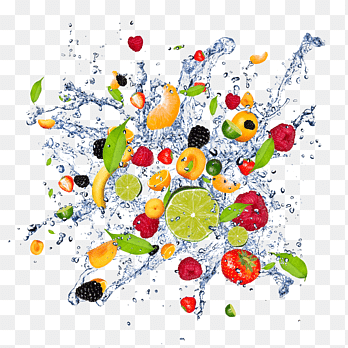
\includegraphics[width=\linewidth]{lemon}
\caption{Fig : LEMON }
\end{subfigure}
\begin{subfigure}{\linewidth}
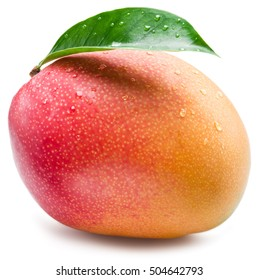
\includegraphics[width=\linewidth]{mango}
\caption{Fig : MANGO}
\end{subfigure}\\


\section{Document Watermarking}
Much of the early work on recognizing the potential
problems with intellectual property rights of digital content and addressing these issues with early watermarking techniques was in the area of document watermarking . These techniques were devised for watermarking electronic versions of text documents which
are in some formatted version such as postscript or PDF.
Most of this work is based on hiding the watermark information into the layout and formatting of the document
directly. In [48]-[50], the authors develop document
watermarking schemes based on line shifts, word shifts as
well as slight modifications to the characters. These techniquesare focused on watermarking the binary-valued
text regions of a document. Watermark detection consists
of postprocessing steps to try to remove noise and correct
for skew. These techniques are quite effective against
some common attacks such as multigenerational photocopying. The authors point out that optical character recognition can remove the layout information and, for suchschemes, remove the watermark information. An openarea of research remains in how to formulate format deviations in a perceptual framework.illustrates an example from  of word shift coding; where
the space has been added before the word “for,” and (b)
contains the unwatermarked and watermarked versions
in their natural state to illustrate that the word shift is not
noticeable. Fig. 5 shows an example from on character alteration for watermark embedding
\section{Graphics Watermarking}
 There has been some work on effective watermarking of
graphics, motivated in part by such standards as
MPEG-4. In [51], the authors address watermarking
three-dimensional polygonal models. The work in [52]
addresses the watermarking of facial animation parame￾ters as defined by the MPEG-4 standard. The watermark
is embedded directly into the parameters and can be ex￾tracted from the watermarked parameters directly or
from video sequences rendered using the parameter bit
stream where the parameters are estimated using a
model-based approach. One bit of watermark information is embedded in a block of facial animation parameter
(FAP) data using a pseudonoise sequence that is generated from the secret key. The authors limit the amount of
deviation the watermark signal has on the FAPs empirically to minimize visible distortion the watermarked FAPs through a traditional correlation detector. The authors demonstrate that they are able to recover the watermark information without error using both the FAPs directly or by estimating them from a
rendered sequence. They also show that their method is
robust to moderate compression using MPEG-2. In gen￾eral, watermarking of graphics data remains an interest￾ing research topic since our understanding of perceptual
models in this domain is not yet fully recognized
\section{Image Watermarking}
\begin{enumerate}
\item Many techniques have been developed for the
watermarking of still image data. For grey-level or
color-image watermarking, watermark embedding techniques are designed to insert the watermark directly into
the original image data, such as the luminance or color
components or into some transformed version of the
original data to take advantage of perceptual properties or
robustness to particular signal manipulations. Requirements for image watermarking include imperceptibility,
robustness to common signal processing operations, and
capacity.

\item Common signal processing operations which
the watermark should survive include compression (such
as JPEG), filtering, rescaling, cropping, A/D and D/A
conversion, geometric distortions, and additive noise.
Capacity refers to the amount of information (or payload) that can be hidden in the host image and detected
reliably under normal operating conditions. Many of the
watermarking techniques are additive, where the water￾mark signal is added directly to the host signal or trans￾formed host signal. The watermark may be scaled
appropriately to minimize noticeable distortions to the
host. Perceptual models may be used to determine and
adapt the watermark scale factor appropriately to the host
data.

\item The watermark itself is a function of the watermark
information, a secret or public key and perhaps the origi￾nal host data. Some examples of watermark information
includes a binary sequence representing a serial number
or credit card number, a logo, a picture, or a signature.
Many of the current watermarking techniques insert one
bit of information over many pixels or transform coeffi￾cients and use classical detection schemes to recover the
watermark information. These types of watermarking
techniques are usually referred to as spread-spectrum approaches, due to their similarity to spread-spectrum com￾munication systems.

\item For still image watermarking,
watermark embedding is applied directly to the pixel values in the spatial domain or to transform coefficients in a
transform domain such as the discrete cosine transform
(DCT) or discrete wavelet transform (DWT). Watermark detection usually consists of some preprocessing
step (which may include removal of the original host sig￾nal if it is available for detection) followed by a correlation
operator
\end{enumerate}
\section{There should be no perceptible difference between the watermarked and original signal}
\begin{itemize}
\item he quality of digital signals is higher than that of their corresponding analogue signals. Traditional assets degrade in quality as time passes. Analogue data require expensive systems to obtain high quality copies, whereas digital data can be easily copied without loss of fidelity.
\end{itemize}\\
\begin{itemize}
\item In this article, we limit the scope of our review to
transparent marking techniques. Transparent
watermarking techniques can be fragile, robust, or
semifragile. Fragile watermarks do not survive lossy transformations to the original host signal and their purpose is
tamper detection of the original signal. There are many
effective ways to insert a fragile watermark into digital
content while preserving the imperceptibility requirement. Placing the watermark information into the perceptually insignificant portions of the data guarantees
imperceptibility and provides fragile marking capabilities. For instance, early watermark techniques for still image data propose inserting watermark information into
the least significant bits of the pixel values. This results in
an imperceptible mark which can detect lossy transformations performed on the watermarked content. For security applications and copyright protection, robust
watermarking techniques have been proposed. Here the
technical challenge is to provide transparency and robustness which are conflicting requirements. Ideally, an effective, robust watermarking scheme provides a mark that
can only be removed when the original content is destroyed as well. The degree of robustness and distortion
necessary to alter the value of the original content can vary
for different applications. Typically, many of the applications for copyright protection involve relatively high
quality original content and the imperceptibility criterion is critical for such application.
\end{itemize}\\

\begin{itemize}
\item In the next section we describe watermarking for different media types including an overview of some sample
algorithms proposed in the literature. This is followed by
a description of a general framework for watermark embedding and watermark detection and decoding, outlining some of the differences for different applications. We
then review some work on modeling the general
watermarking problem and drawing parallels to communication and information theory to help understand the
fundamental properties and limitations of a watermarking system. This work is very useful for future algorithm
design and helping to define open areas of research.
Lastly, we review and summarize future directions in this
new and exciting area.
\end{itemize}\\

\section{Audio Watermarking}
\begin{enumerate}
\item Most of the research on audio watermarking has been focused on either direct watermarking of the audio signal or
bit stream embedding where the audio is represented in a
compressed format. Just as in image and video
watermarking, the use of perceptual models is an important component in generating an effective and acceptable
watermarking scheme for audio.

\item Many of the requirements for audio watermarking are similar to image watermarking, such as inperceptibility (inaudibility), robustness to signal alterations such as compression,filtering, and A/D and D/A conversion.
\item  The Secure Digital Music Initiative (SDMI) that consists of companies and organizations in information technology, consumer electronics, security technology, the
recording industry, and ISPs has been formed to examine
technology which provides some security features for
digital music and copyright protection for
next-generation portable digital music devices. Phase I
screening looks for a watermark in the content but allows
all music that is compatible with the device to be playable.
Phase II will incorporate watermark detection which will
allow new releases to play while filtering out pirated copies of music. After extensive testing of imperceptibility
and robustness, SMDI has chosen ARIS audio
watermarking technology for Phase I screening technology which will be used to indicate when the software used
by Phase I devices should be upgraded to incorporate
Phase II technology. Some of the requirements particular
to music as seen by the SDMI group includes inaudibility,
robustness, tamper resistance, reliability (no false
positives), ease of implementation, cost, and ability to
compress the content.
\end{enumerate}
\centering
\begin{subfigure}{\linewidth}
\includegraphics[width=\linewidth]{picture audio}
\end{subfigure}\\
\begin{subfigure}{\linewidth}

\includegraphics[width=\linewidth]{video}
\caption{Fig :AUDIO }
\end{subfigure}\\
\section{Watermark Embedding}
The watermark embedding scheme can either embed the
watermark directly into the host data or to a transformed
version of the host data. Some common transform domain watermarking for image data can be DCT based [7],
[34], [65], [16], [17], [38] or wavelet based [18], [7].
Transform-domain techniques are popular due to the
natural framework for incorporating perceptual knowledge into the embedding algorithm and because many of
the state-of-the-art compression techniques such as JPEG
work in the same framework (block-based DCT) and this
allows for watermarking of the compressed bit stream
with only partial decoding. A simple way of applying
some perceptual knowledge is to watermark the
midfrequency components, since the low frequency components are very sensitive to distortion and the high frequency components can be removed without significantly affecting the original image quality. Use of more formal perceptual models for watermark embedding have also been developed. The earliest watermarking techniques involved embedding a low energy pseudorandom noise pattern directly to the digital host signal .A basic block diagram of a watermark system is illustrated in Fig. 1 where S denotes the original host signal
and can represent image luminance values or some transform domain signal such as the DCT coefficients. M denotes the watermark message which, for example, can be a sequence of bits representing a serial number or credit card number, one bit in the case of a signature for authentication applications, a logo or picture. When the message M is used to identify the destination or end-user to help track illegal usage later, M is sometimes referred to as a
fingerprint and recovering M is known as identification.
The watermark signal can either represent a signature
where the goal is to determine whether or not the signature is present in the content (detection or verification) or a
sequence of information bits or other data where the goal
is to extract the bit pattern with low probability of bit error or to identify one out of N possible watermark messages. The watermark can be binary or real valued. The
watermark is usually parameterized by a keyK which is secret and could be used to generate a random sequence to. This key could also be used to determine a random sequence which identifies locations in the host signal for watermark embedding. Without knowledge of the key, it should be difficult to remove or alter the embedded message without destroying the original content.
For many applications, just as in cryptography,
watermarking algorithms follow Kerckhoff’s principle,
that is, the watermark embedding process is public and
security is based only on choosing a secret key. The watermark information or key could also be dependent on the
host signal. For instance, the secret key may depend on a
hash of the host signal.
\section{Watermark Detection}
In keeping consistent with the taxonomy of earlier detection and estimation problems, we differentiate between
detection and identification at the watermark receiver.
Detection or verification refers to the process of making a
binary decision at the decoder—whether a specific watermark is or is not present in the received data. This may be
appropriate for authentication applications where you
would like to verify that a signature is present in the received content. This problem lends itself to a hypothesis
testing formulation, and the effectiveness of the watermark scheme can be measured in terms of Type I and Type
II errors. Type I errors or false positives refer to the case
where a watermark is detected when it does not exist, and
Type II errors or false negatives refer to the case when an
existing watermark is not detected. For many applications, especially in the consumer markets, it is more important to have low or zero false positives at the risk of
higher false negatives rates. This is also referred in the literature as the probability of false alarm and probability of
detection. Plots of probability of detection versus the
probability of false alarm are referred to as receiver oper￾ating characteristics (ROC) curves.Identification refers to
the process of being able to decode one of N possible
choices (messages) at the receiver. An application for this
includes copyright protection where multiple copies of
the same content get a unique label so that misuse of one
of the copies can be traced back to its owner. Identifica￾tion problems can be categorized as “open set” or “closed
set.” Open set identification refers to the possibility that
one of N or no watermark exists in the data. Closedset refers to problems where one of N possible watermarks is
known to be in the received data and the detector has to
pick the most likely one. For identification problems
where the goal is to extract a watermark sequence, for instance a binary sequence of length B where one of N B =2
watermark patterns is present, the bit error rate (BER) is
a very useful measure of performance. The effectiveness
of a watermarking scheme can be illustrated by plotting
the BER versus SNR in the case of an additive noise
watermarking attack as shown in Fig. 6. In this example,
32 bits of watermark information were inserted into the
“Lena” image with a simple repetition code for protection. The effectiveness of the watermarking scheme was
tested by detecting the bits in the presence of an additive
noise attack (this is a good model for some common
transformations such as compression.
\section{Fundamental Properties and Limitations of Watermarking}
\begin{itemize}
\item Much of the work on trying to model and understand
some of the fundamental properties and limitations of
watermarking algorithms is based on drawing parallels to
communications systems. We have already mentioned
that many of the popular watermark embedding algorithms are variations on the idea of spread-spectrum techniques for secure communication systems where an
information bearing narrowband signal is converted into
a wideband signal prior to transmission, by modulating
the information waveform with a wideband noiselike
waveform. As a result of the bandwidth expansion, within
any narrow spectral band, the total amount of energy
from the information signal is small. By appropriately
combining all the weak narrowband signals at the demodulator, the original information signal is recovered

\item There has been some interesting work in trying to
model and understand some of the fundamental properties and limitations of watermarking algorithms. An information theoretic analysis of
watermarking is presented [78] where an elegant framework is proposed for the hiding capacity problem (water￾mark payload). The framework shows the tradeoff
between achievable information hiding rates and allowed
distortions for the information hider (watermark
embedder) and the attacker (possible distortions to remove or alter the watermark)
\end{itemize}
\section{CONCLUSION}
 We have reviewed the basic watermarking algorithms as
they apply to different applications and media types. Although many technical problems have been addressed,
there are many more yet to be solved. Many of the techniques developed for watermarking are based on a solid
understanding of communications and signal processing
principles, but there are still many technical challenges to
be solved. It is difficult to model the distortions intro￾duced by common signal processing transformations,
which either intentionally or unintentionally affect the
watermark detection or identification capabilities. Al￾though very nice work exists in trying to understand the
fundamental limitations of watermark embedding and
detection, attack channels such as geometrical distortions
cannot be described by these models. Other areas have
not been resolved as well. Besides the obvious caveat of
whether watermarking technology will be effective in a
court of law, other questions remain. What are reasonable
distortions for particular applications that the watermark
is expected to survive? What is a meaningful measure of
distortion that can be used to determine the effectiveness
of a watermarking scheme? How is monitoring and policing for copyright infringement done? How much are potential customers for watermarking technology willing to
pay for it?
These questions and many interesting technical chal￾lenges remain in this new and exciting field. The overview
we have presented is meant to summarize the salient features and directions of watermarking research and technology and the interested reader is encouraged to explore
the references for more details.\\ \\
\section{REFERENCE}
\begin{enumerate}
\item Special Issue on Copyright and Privacy Protection, IEEE J. Select. Areas Commun., vol. 16, May 1998.\\
\item Special Issue on Identification and Protection of Multimedia Information,Proc. IEEE, vol. 87, no. 7, July 19999\\
\item “IS&T and SPIE electronic imaging,” presented at the Conference on Secu￾rity and Watermarking of Multimedia Contents, San Jose, CA, 1999, 2000.\\
\item Erlangen Watermarking Workshop, Erlangen, Germany, 5-6 Oct. 1999.\\
\item International Workshop on Information Hiding, 1996.
\end{enumerate}
\end{document}